\documentclass[UTF8]{beamer}
\usepackage{ctex, hyperref}
\usepackage[T1]{fontenc}
\usepackage{fontspec}
\usepackage[utf8]{inputenc}
\usepackage{amsmath,amsthm}
\usepackage{amssymb,amsfonts}
\usepackage{mathrsfs,bm}
\usepackage[linesnumbered,algoruled,boxed,lined]{algorithm2e} %环境

% other packages
\usepackage{latexsym,amsmath,xcolor,multicol,booktabs,calligra}
\usepackage{graphicx,pstricks,listings,stackengine}
\usepackage{auto-pst-pdf}


\author{分享人:孟凡辉 }
\title{《一阶复本对称破缺理论》}
\subtitle{PART V~~~Chap. 19}
\institute{中山大学    \textrm{COIN Lab}}
\date{\textrm{2023}年\textrm{03}月\textrm{01}日}
\usepackage{SYSUBeamer}

% defs
\def\cmd#1{\texttt{\color{red}\footnotesize $\backslash$#1}}
\def\env#1{\texttt{\color{blue}\footnotesize #1}}
\definecolor{deepblue}{rgb}{0,0,0.5}
\definecolor{deepred}{rgb}{0.6,0,0}
\definecolor{deepgreen}{rgb}{0,0.5,0}
\definecolor{halfgray}{gray}{0.55}

\lstset{
    basicstyle=\ttfamily\small,
    keywordstyle=\bfseries\color{deepblue},
    emphstyle=\ttfamily\color{deepred},    % Custom highlighting style
    stringstyle=\color{deepgreen},
    numbers=left,
    numberstyle=\small\color{halfgray},
    rulesepcolor=\color{red!20!green!20!blue!20},
    frame=shadowbox,
}


\begin{document}

\kaishu

\begin{frame}
  \titlepage
  \begin{figure}[htpb]
    \begin{center}
      
\includegraphics[width=0.2\linewidth]{pic/SYSU_Log.jpg}
    \end{center}
  \end{figure}
\end{frame}

\begin{frame}
  \tableofcontents[sectionstyle=show,subsectionstyle=show/shaded/hide,subsubsectionstyle=show/shaded/hide]
\end{frame}


\section{Background}

\begin{frame}{Background}
  \begin{minipage}[c]{1.0\linewidth}
    一阶复本对称破缺(one-step replica symmetry breaking, 1RSB)理论的由来: {\color{red} 解决``负熵''危机.}
  \end{minipage}
  \vfill
  \begin{minipage}[c]{0.3\linewidth}
    \begin{figure}
      \centering
      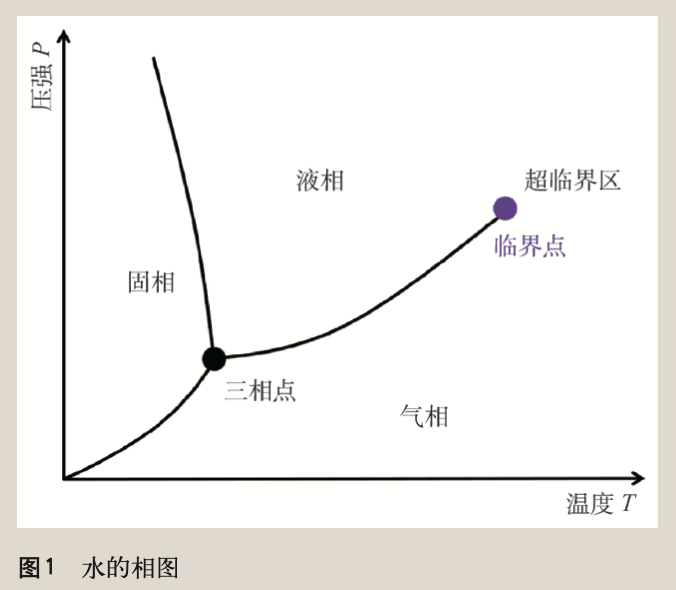
\includegraphics[width=0.8\linewidth]{./fig/水的相图.png}
    \end{figure}
  \end{minipage}
  \hfill
  \begin{minipage}[c]{0.3\linewidth}
    \begin{figure}
      \centering
      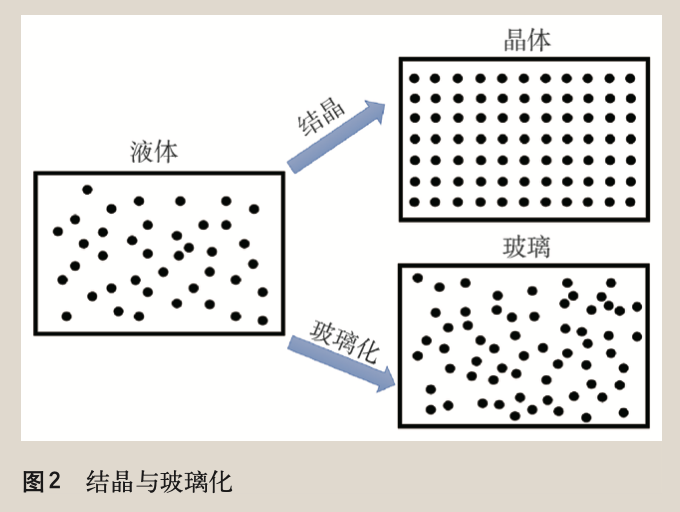
\includegraphics[width=0.9\linewidth]{./fig/结晶与玻璃化.png}
    \end{figure}
  \end{minipage}
  \hfill
  \begin{minipage}[c]{0.3\linewidth}
    \begin{figure}
      \centering
      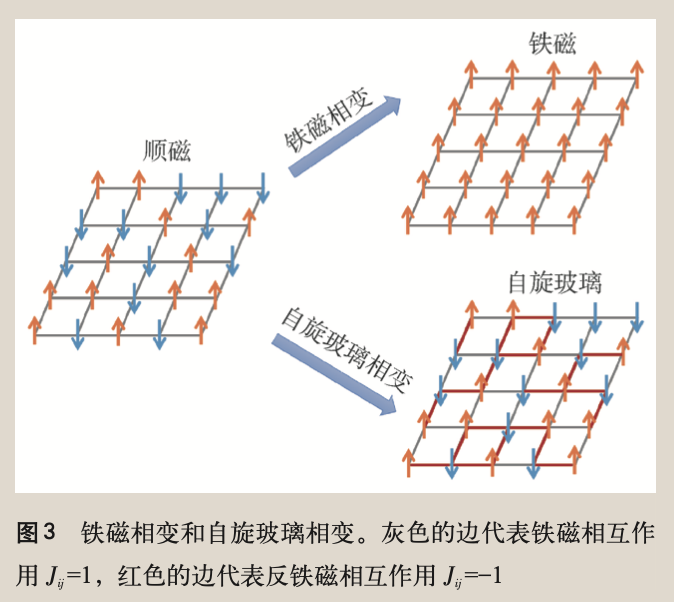
\includegraphics[width=0.8\linewidth]{./fig/相变.png}
    \end{figure}
  \end{minipage}
  \vfill
  \begin{minipage}[c]{0.3\linewidth}
    \small
    \begin{equation}
      \left[ \log Z \right] = \lim_{n \rightarrow 0} \frac{\left[ Z^n \right] - 1}{n} \notag
    \end{equation}
    \begin{equation}
      q_{\alpha \beta} = \frac{1}{N} \sum_{i=1}^{N} \left[ m_{i}^{\alpha} m_{i}^{\beta} \right] \notag
    \end{equation}
  \end{minipage}
  \hfill
  \begin{minipage}[c]{0.3\linewidth}
    \begin{figure}
      \centering
      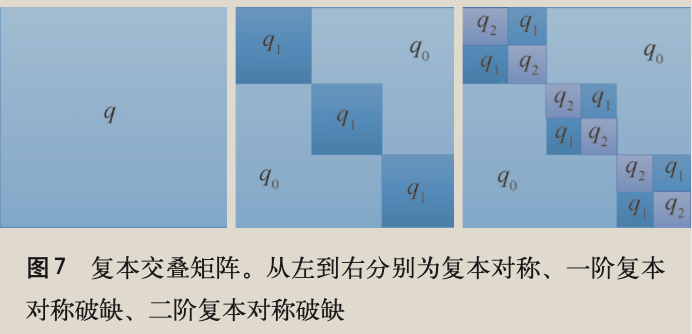
\includegraphics[width=1.0\linewidth]{./fig/复本交叠矩阵.png}
    \end{figure}
  \end{minipage}
  \hfill
  \begin{minipage}[c]{0.3\linewidth}
    \begin{figure}
      \centering
      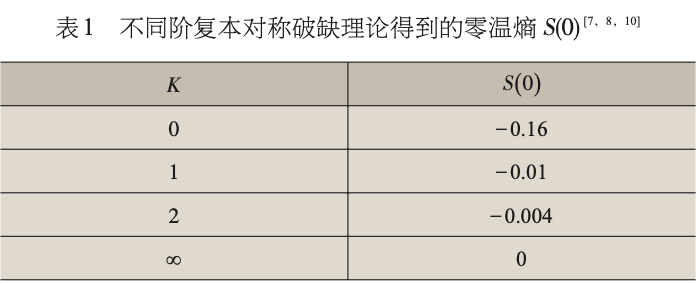
\includegraphics[width=1.0\linewidth]{./fig/零温熵.png}
    \end{figure}
  \end{minipage}
\end{frame}

\begin{frame}{Background}
  \begin{minipage}[c]{0.9\linewidth}
    消息传递(message passing)算法的局限性.
  \end{minipage}
  \vfill
  \begin{minipage}[c]{0.9\linewidth}
    \begin{figure}
      \centering
      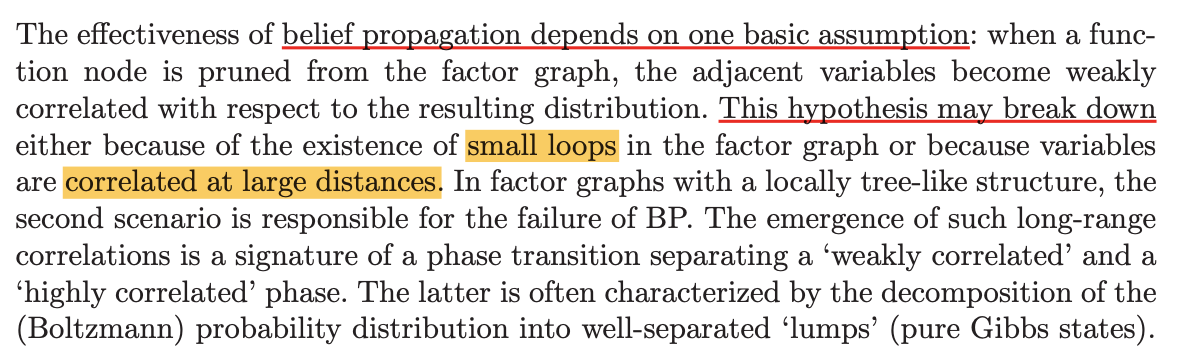
\includegraphics[width=0.8\linewidth]{./fig/BP_limitation.png}
    \end{figure}
  \end{minipage}
  \vfill
  \begin{minipage}[c]{0.9\linewidth}
    \begin{figure}
      \centering
      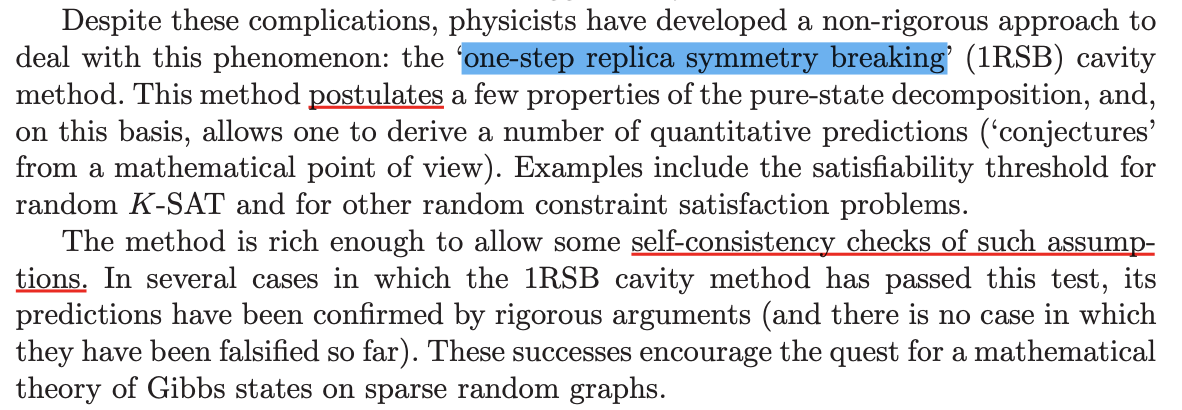
\includegraphics[width=0.8\linewidth]{./fig/1RSB.png}
    \end{figure}
  \end{minipage}
  \vfill
  \begin{minipage}[c]{0.9\linewidth}
    \begin{figure}
      \centering
      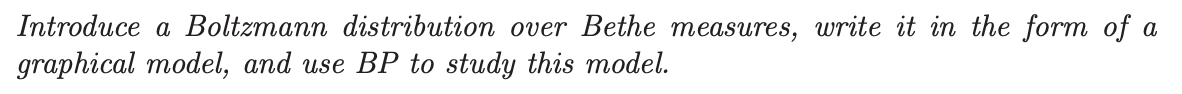
\includegraphics[width=0.8\linewidth]{./fig/1RSB_summary.png}
    \end{figure}
  \end{minipage}
\end{frame}


\section{Beyond BP: Many states}

\begin{frame}{BP equations}
  \begin{minipage}[c]{0.9\linewidth}
    \begin{figure}
      \centering
      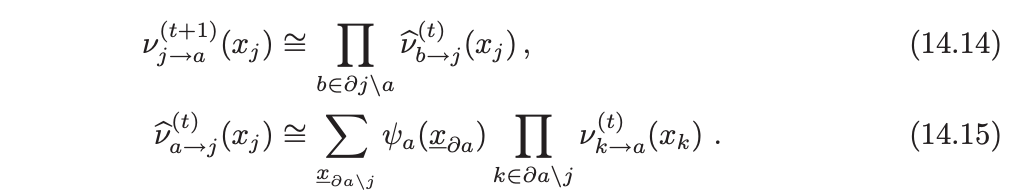
\includegraphics[width=0.9\linewidth]{./fig/BP_equations.png}
    \end{figure}
  \end{minipage}
  \vfill
  \begin{minipage}[c]{0.9\linewidth}
    \begin{figure}
      \centering
      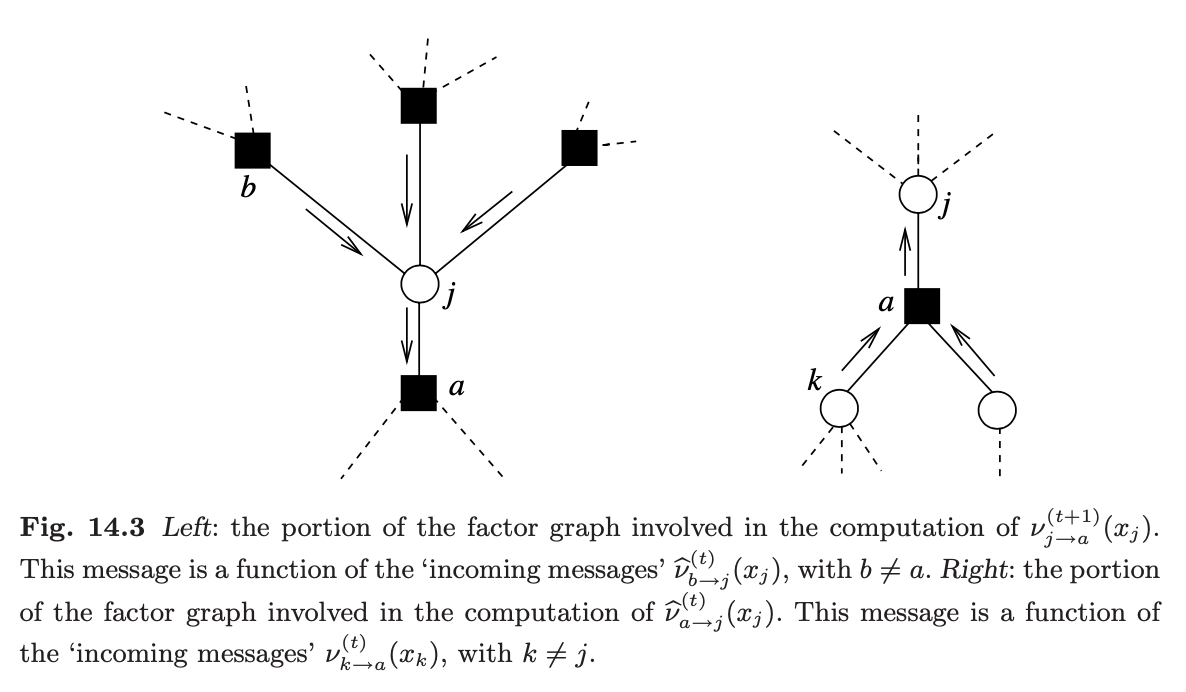
\includegraphics[width=0.9\linewidth]{./fig/Factor_graph.png}
    \end{figure}
  \end{minipage}
\end{frame}

\begin{frame}{Bethe measures}
  \begin{minipage}[c]{0.9\linewidth}
    \begin{figure}
      \centering
      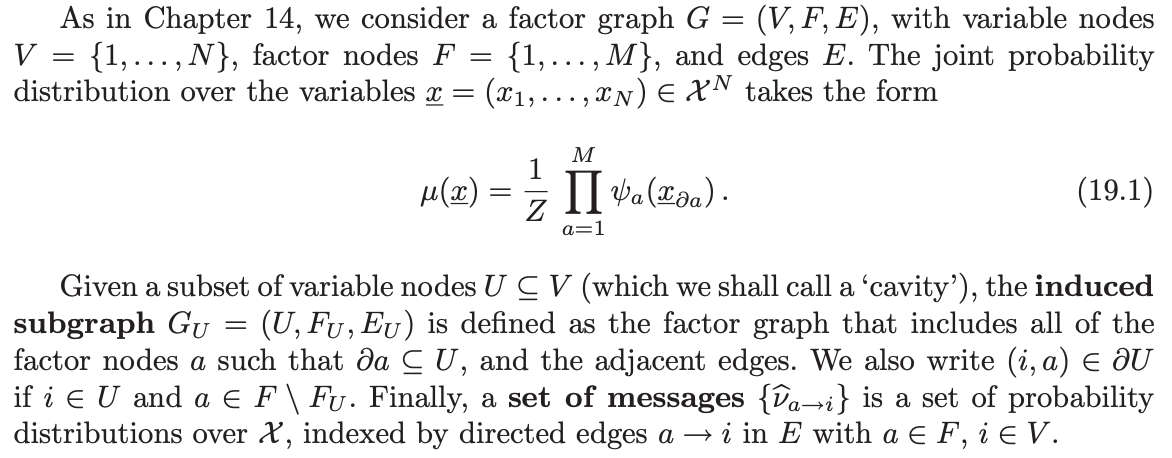
\includegraphics[width=0.9\linewidth]{./fig/Eq_191.png}
    \end{figure}
  \end{minipage}
  \vfill
  \begin{minipage}[c]{0.9\linewidth}
    \begin{figure}
      \centering
      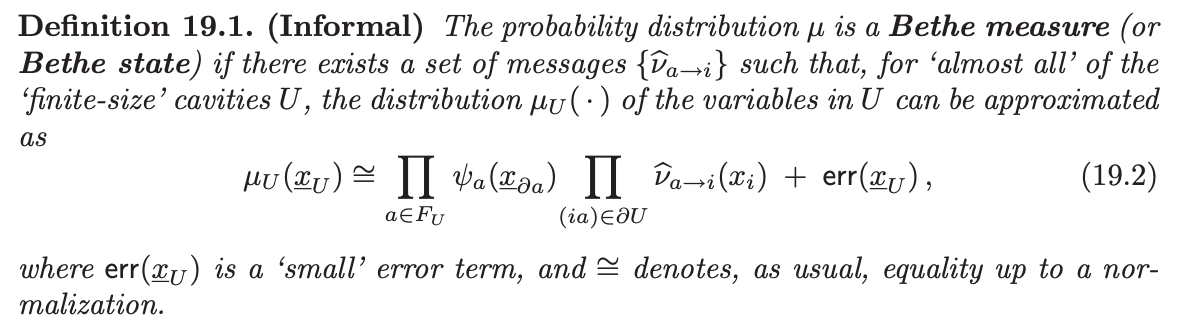
\includegraphics[width=0.9\linewidth]{./fig/Eq_192.png}
    \end{figure}
  \end{minipage}
\end{frame}

\begin{frame}{Example 1}
  \begin{minipage}[c]{0.9\linewidth}
    \begin{figure}
      \centering
      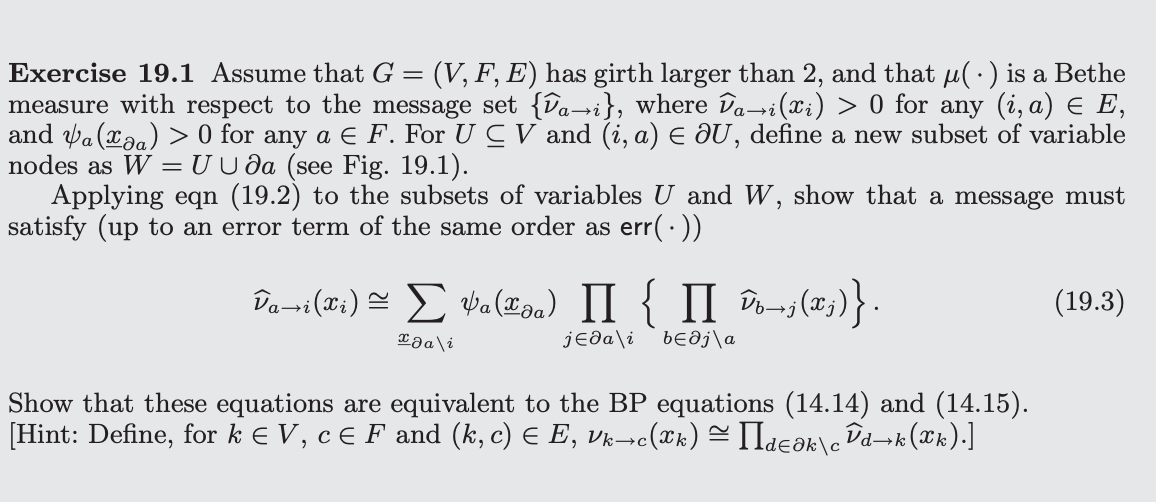
\includegraphics[width=0.85\linewidth]{./fig/Exam_191.png}
    \end{figure}
  \end{minipage}
  \vfill
  \begin{minipage}[c]{0.9\linewidth}
    \begin{figure}
      \centering
      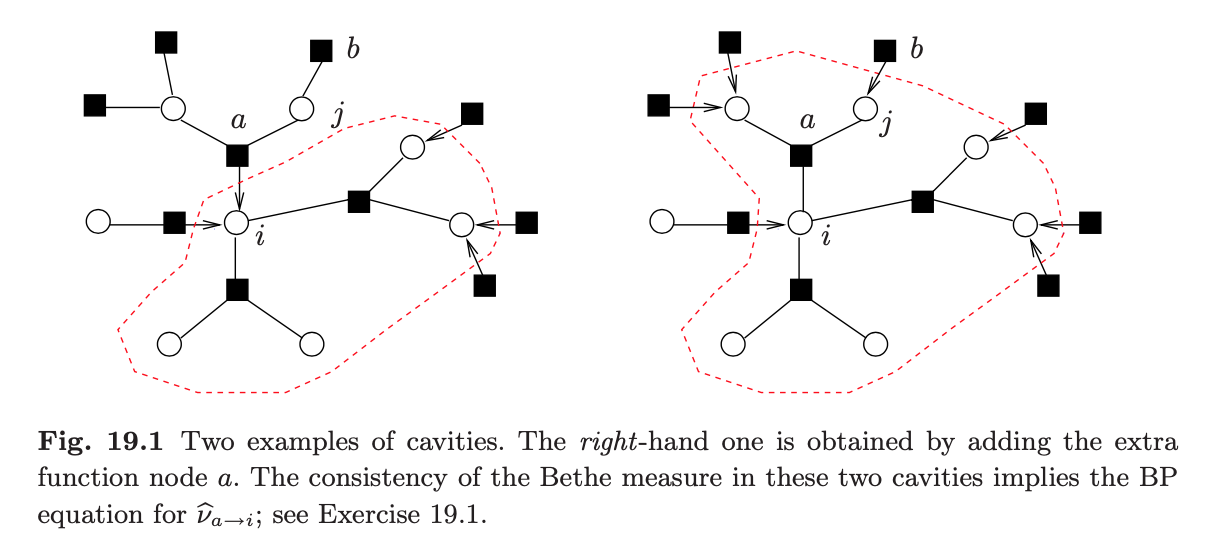
\includegraphics[width=0.8\linewidth]{./fig/FIG_191.png}
    \end{figure}
  \end{minipage}
\end{frame}

\begin{frame}{Example 2}
  \begin{minipage}[c]{0.9\linewidth}
    \begin{figure}
      \centering
      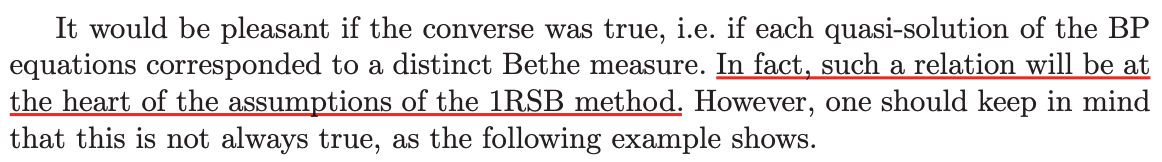
\includegraphics[width=0.9\linewidth]{./fig/Exception.png}
    \end{figure}
  \end{minipage}
  \vfill
  \begin{minipage}[c]{0.9\linewidth}
    \begin{figure}
      \centering
      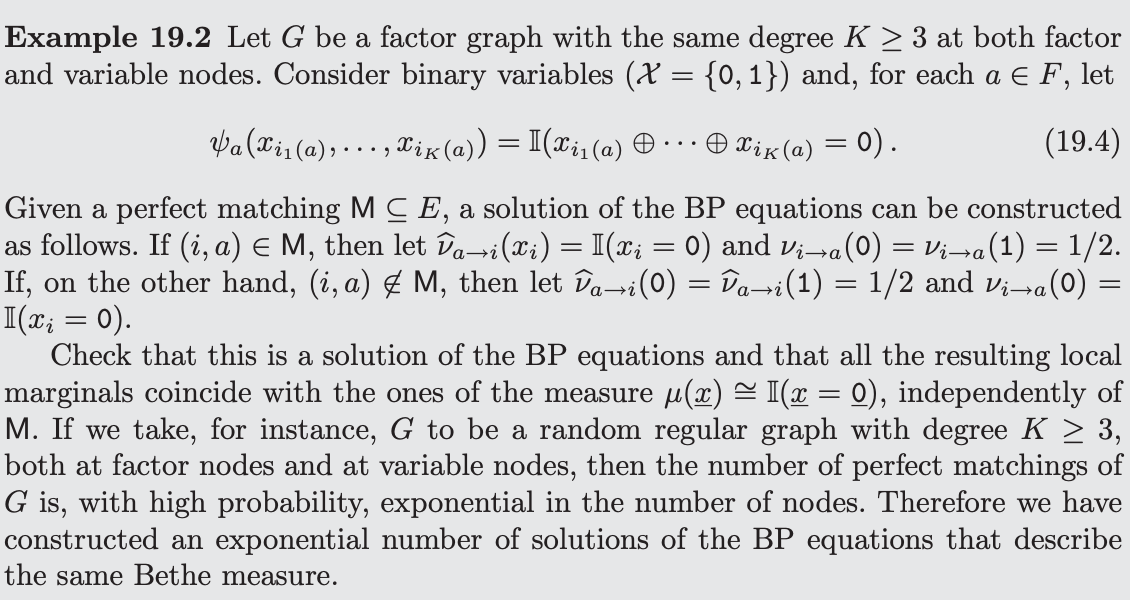
\includegraphics[width=0.85\linewidth]{./fig/Exam_192.png}
    \end{figure}
  \end{minipage}
\end{frame}

\begin{frame}{Generic scenarios}
  \begin{figure}
    \centering
    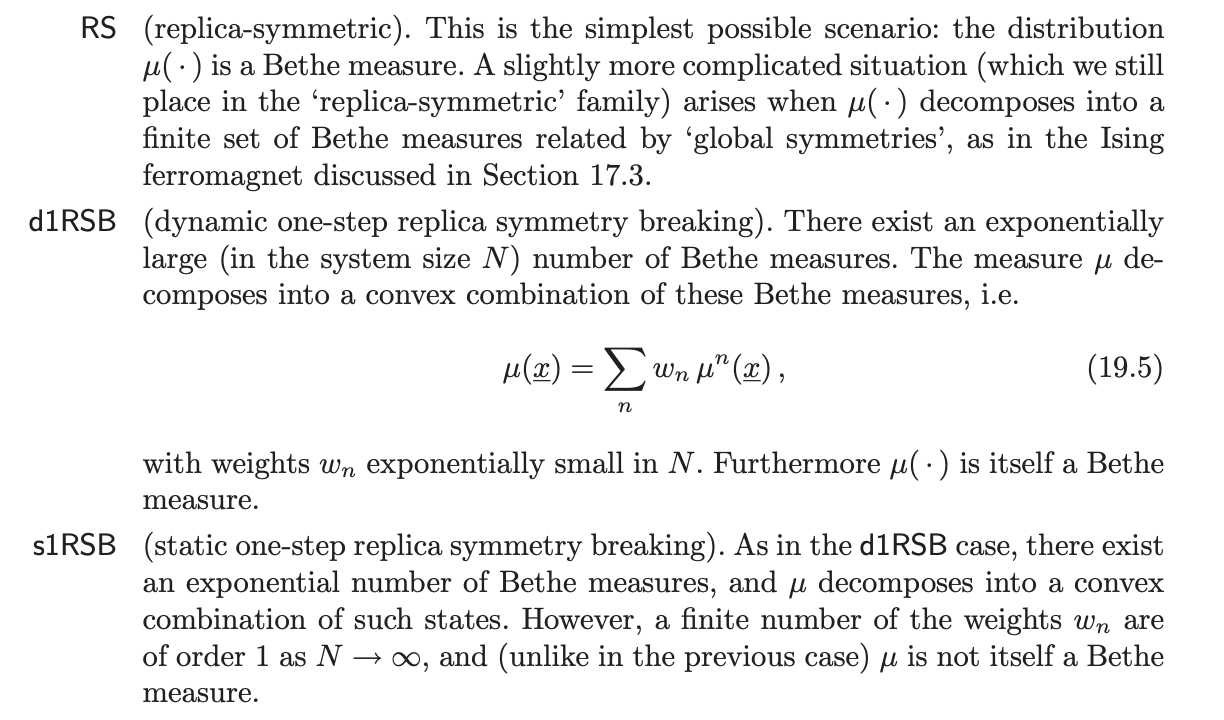
\includegraphics[width=0.9\linewidth]{./fig/Generic_Scenarios.png}
  \end{figure}
\end{frame}

\begin{frame}{Three assumptions}
  \begin{minipage}[c]{0.9\linewidth}
    \begin{figure}
      \centering
      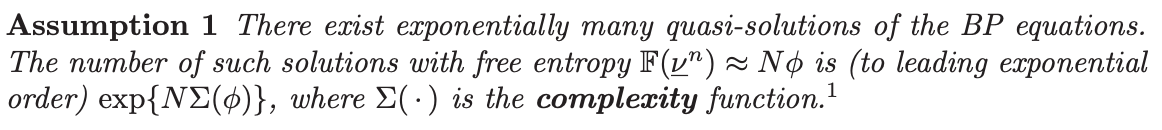
\includegraphics[width=0.9\linewidth]{./fig/Assume_1.png}
    \end{figure}
  \end{minipage}
  \vfill
  \begin{minipage}[c]{0.9\linewidth}
    \begin{figure}
      \centering
      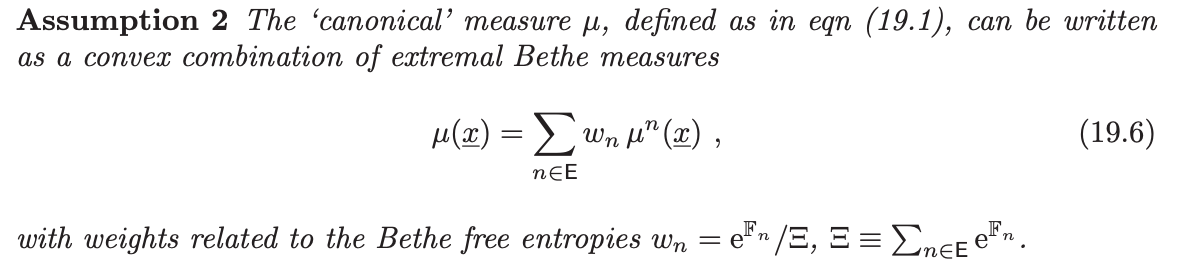
\includegraphics[width=0.9\linewidth]{./fig/Assume_2.png}
    \end{figure}
  \end{minipage}
  \vfill
  \begin{minipage}[c]{0.9\linewidth}
    \begin{figure}
      \centering
      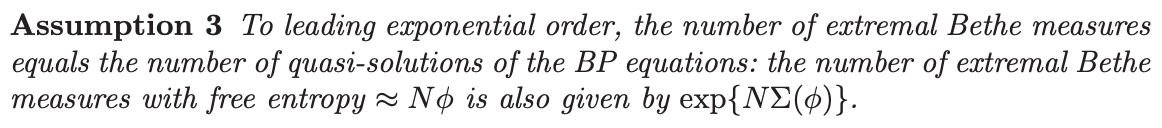
\includegraphics[width=0.9\linewidth]{./fig/Assume_3.png}
    \end{figure}
  \end{minipage}
\end{frame}


\section{1RSB cavity equations}

\begin{frame}{Generalized partition function}
  \begin{figure}
    \centering
    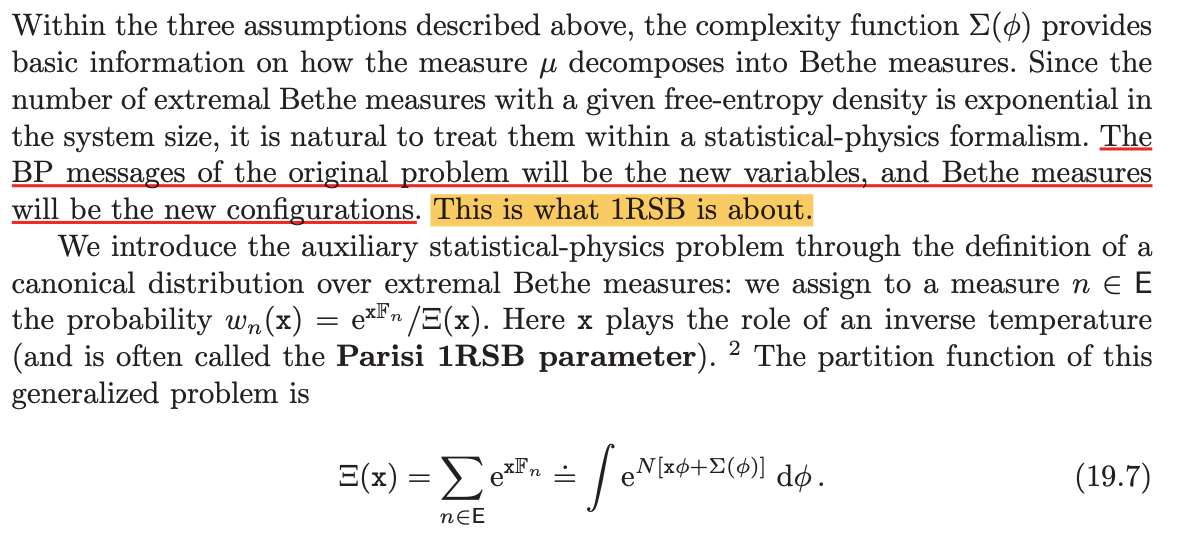
\includegraphics[width=0.9\linewidth]{./fig/Eq_197.png}
  \end{figure}
\end{frame}

\begin{frame}{Free energy landscape}
  \begin{figure}
    \centering
    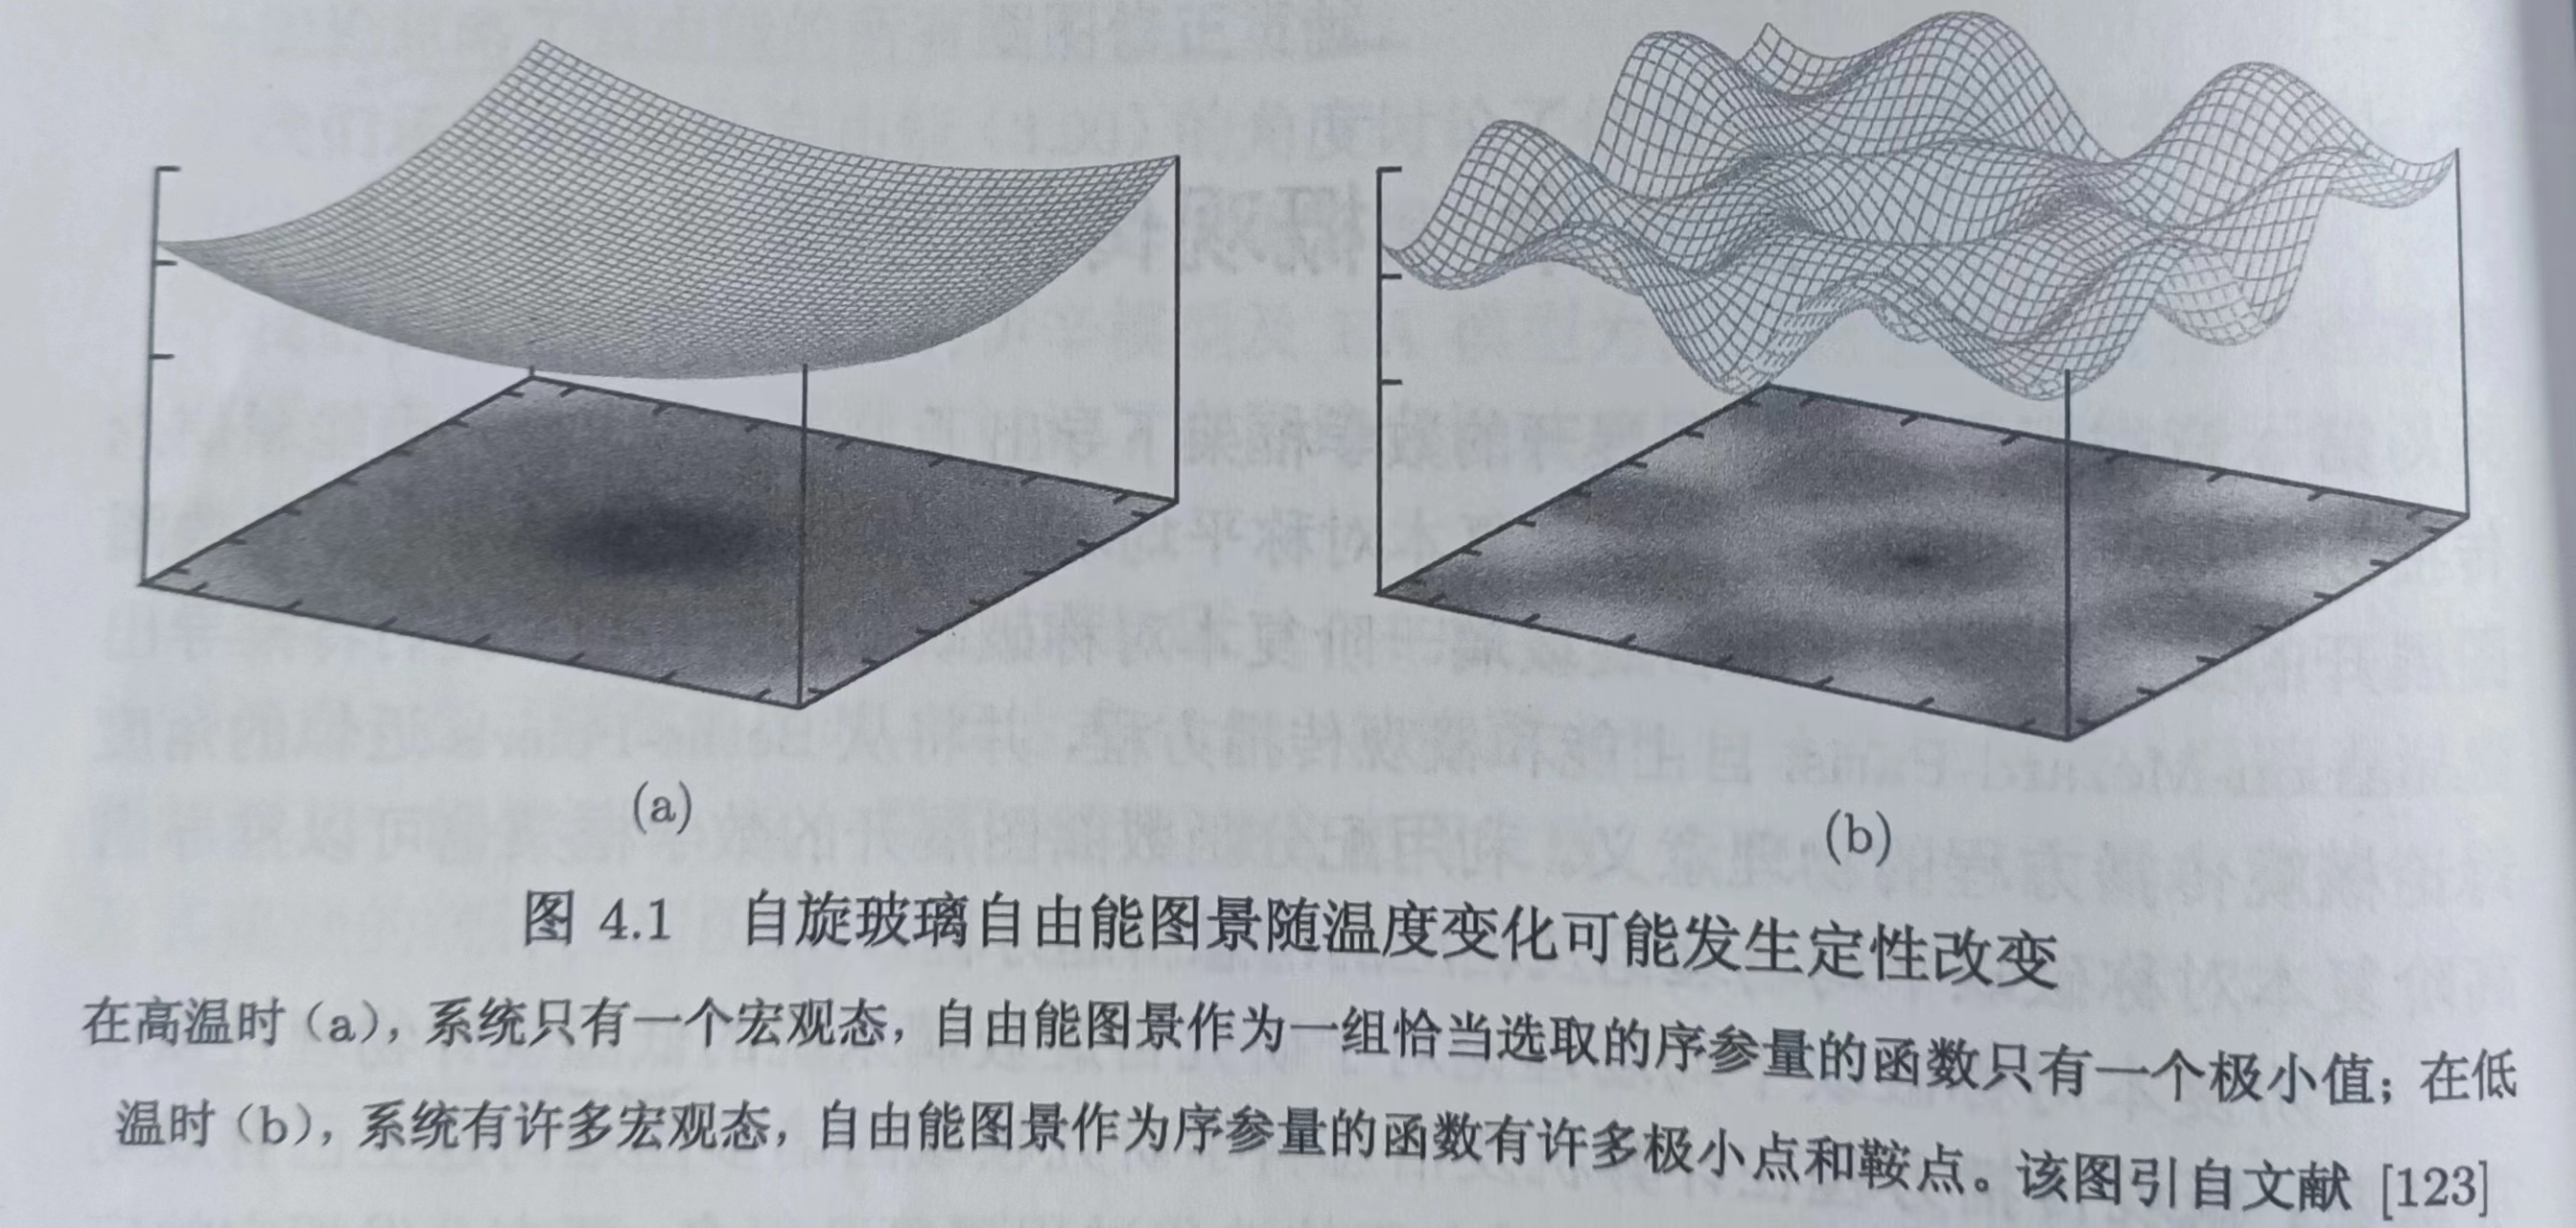
\includegraphics[width=0.9\linewidth]{./fig/FreeEnergy_Landscape.jpg}
  \end{figure}
\end{frame}

\begin{frame}
  \begin{minipage}[c]{0.48\linewidth}
    \begin{figure}
      \centering
      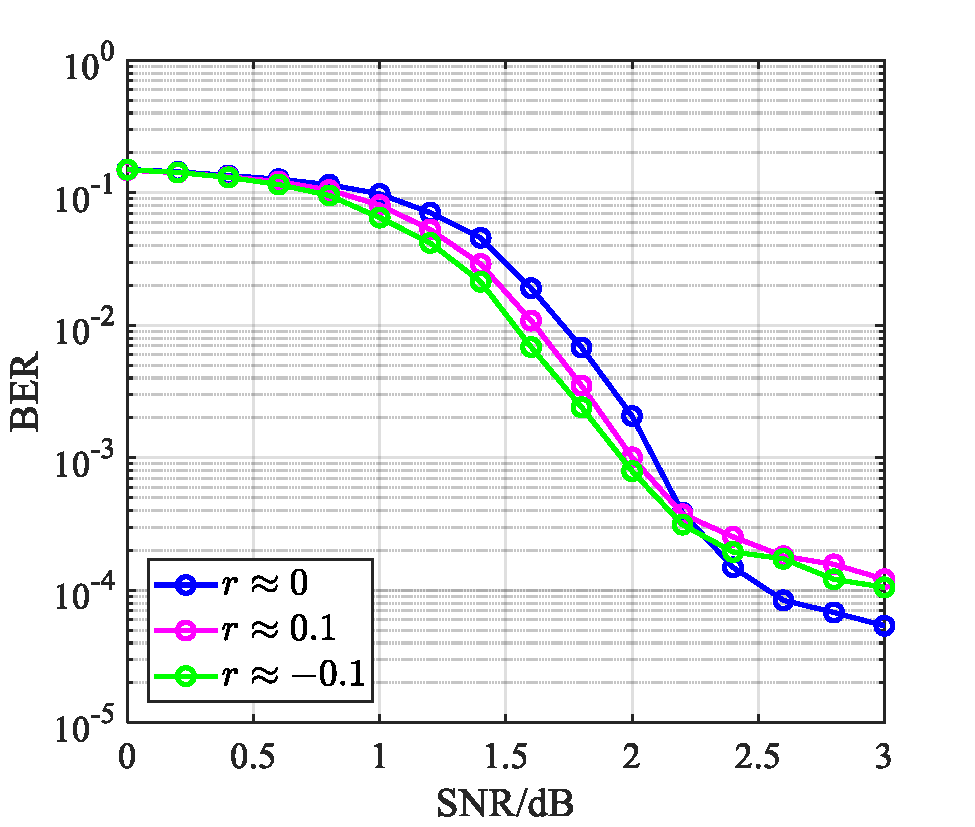
\includegraphics[width=0.95\linewidth]{./fig/BER_DegCorr.pdf}
    \end{figure}
  \end{minipage}
  \hfill
  \begin{minipage}[c]{0.48\linewidth}
    \begin{figure}
      \centering
      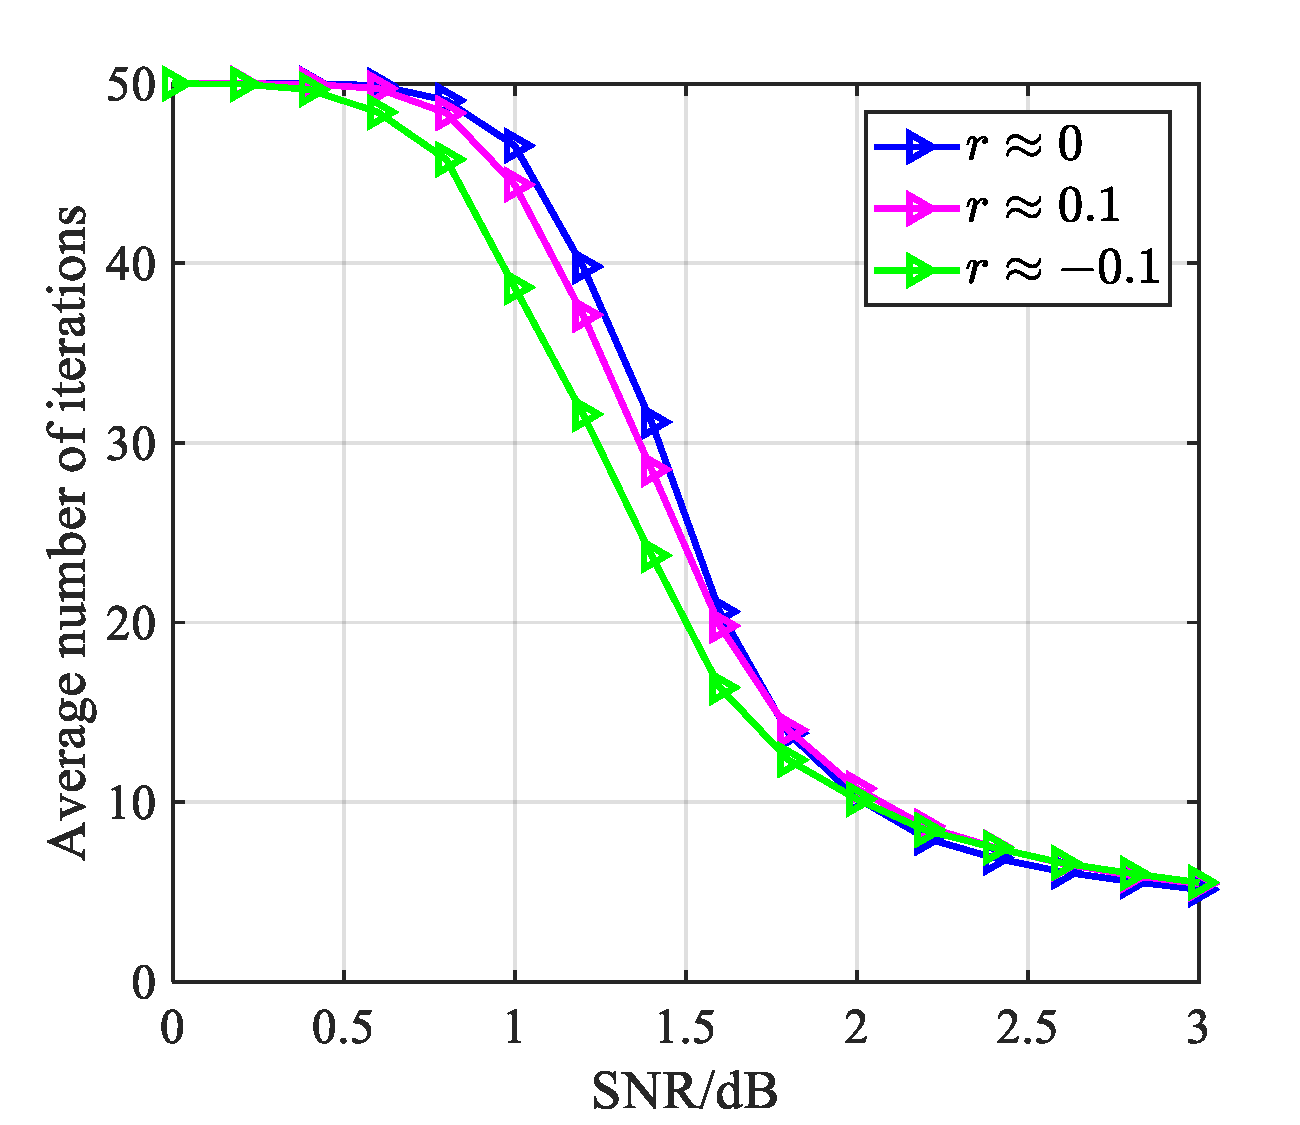
\includegraphics[width=0.95\linewidth]{./fig/ITER_DegCorr.pdf}
    \end{figure}
  \end{minipage}
\end{frame}

\begin{frame}
  \begin{center}
    {\Huge\calligra Thanks!}
  \end{center}
\end{frame}

\end{document} 